\documentclass{beamer}

\mode<presentation>{
  \usetheme{Warsaw}
}


\usepackage[spanish,es-tabla,es-nodecimaldot]{babel}
\usepackage{tikz}
\usepackage{pgf}  %Para realizar figures
\usepackage{xcolor} % Para los colores
\usepackage{enumerate}
\usepackage{graphicx}
\usepackage{array}
\usepackage{cancel}
\usepackage{amssymb}
\usepackage{hyperref}
\usepackage{tcolorbox}  %Cuadros de teoremas


\title[ \hspace{21mm} \insertframenumber \ de \inserttotalframenumber ]
{T\'ecnicas de conteo}

\subtitle
{Probabilidad, procesos aleatorios e inferencia}

\author[]
{Ana Maritza Bello Yañez}


\institute[Instituto Polit\'ecnico Nacional]
{
  \inst{1}
  Centro de Investigaci\'on en Computaci\'on
  }

\date[Short Occasion]
{\today}

\keywords{conteo, permutaci\'on, combinaci\'on, variaci\'on, factorial}

\begin{document}

\begin{frame}
  \titlepage
\end{frame}


\begin{frame}{Regla de multiplicaci\'on}
  \onslide <1->
  \begin{block}{}
    Si queremos contar el n\'umero de formas en las que pueden ocurrir dos eventos
    simult\'aneos, podemos hacerlo usando la regla de la multiplicaci\'on.
  \end{block}

  \onslide <2->
  \begin{block}{Regla}
    Si un evento puede ocurrir de $n_1$ formas diferentes, y para cada una de
    \'estas puede ocurrir un segundo evento simultaneo en $n_2$ formas diferentes, entonces los
    dos eventos pueden ocurrir de $n_1*n_2$ formas diferentes.
  \end{block}

  \onslide <3->
  As\'i, para una serie de $k$ eventos tenemos:

  \begin{block}{}
    \begin{equation}
      n_1*n_2*n_3*...*n_k
    \end{equation}
  \end{block}

  \onslide <4->
  Ejemplo:
  
  \begin{figure}
    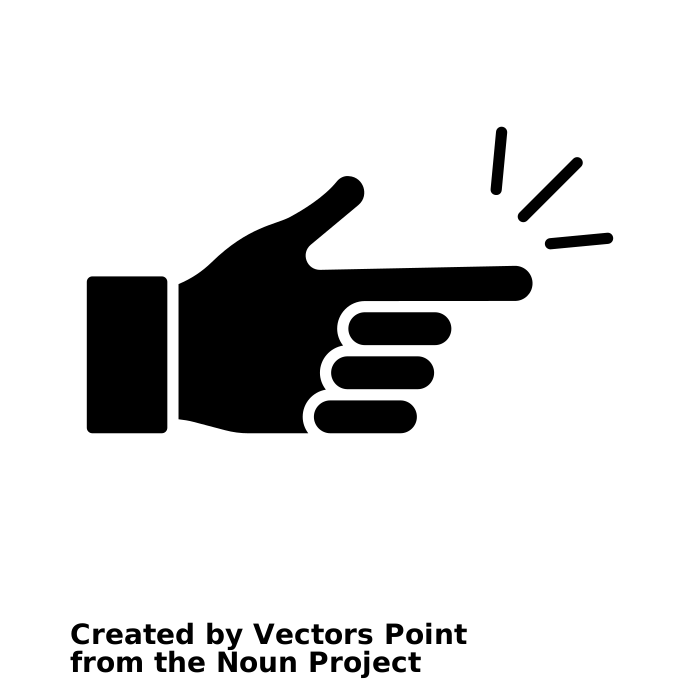
\includegraphics[width=2cm,angle=0,trim={1mm 170mm 1mm 250mm},clip]{figures/example-finger.png}
  \end{figure}

\end{frame}

\begin{frame}{Ejemplo de regla de multiplicaci\'on}
  \transdissolve
  \transblindshorizontal<3-4>
  \transwipe[duration=5]<5-6>

  \onslide <1->
  \begin{exampleblock}{}
    \begin{figure}
      \raggedleft
      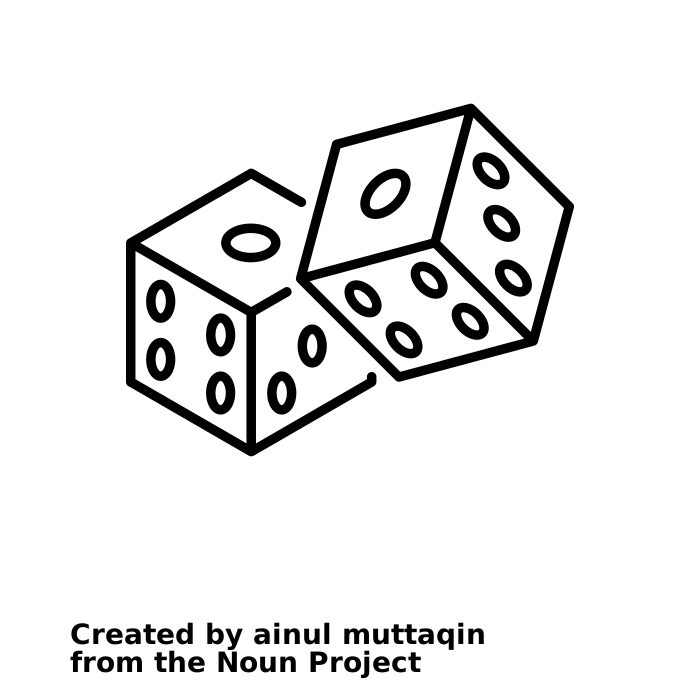
\includegraphics[width=2cm,angle=0,trim={1mm 210mm 1mm 200mm},clip]{figures/dice-roll.png}
    \end{figure}

    {¿De cuantas formas diferentes pueden caer dos dados \\
    de 6 caras si se lanzan al mismo tiempo?}
  \end{exampleblock}

    \vfill
    \onslide <2->{Soluci\'on:}
    \vfill
    \onslide <3->{El primer dado puede caer en cualquiera de $n_1 = 6$ maneras.}
    \vfill
    \onslide <4->{Para cada una de esas 6 maneras el segundo dado tambi\'en puede caer en $n_2 = 6$ formas.}
    \vfill
    \onslide <5->{Por lo tanto, el par de dados puede caer en $n_1*n_2 = (6)*(6) = 36$ formas posibles.}
  
\end{frame}

\begin{frame}{Diagrama de \'arbol}
  \begin{columns}
    \column{.5\textwidth}
      \begin{block}{}
        \begin{itemize}
          \onslide <1-> \item Los diagramas de \'arbol muestran todos los resultados posibles de un
          evento.
          \onslide <2-> \item Cada rama en un diagrama de \'arbol representa un posible resultado. 
          \onslide <3-> \item Los diagramas de \'arbol pueden usarse para encontrar el n\'umero de
          resultados posibles y calcular la probabilidad de los posibles resultados.
        \end{itemize}
      \end{block}

    \onslide <1->
    \column{.5\textwidth}
      \begin{figure}
        \centering
        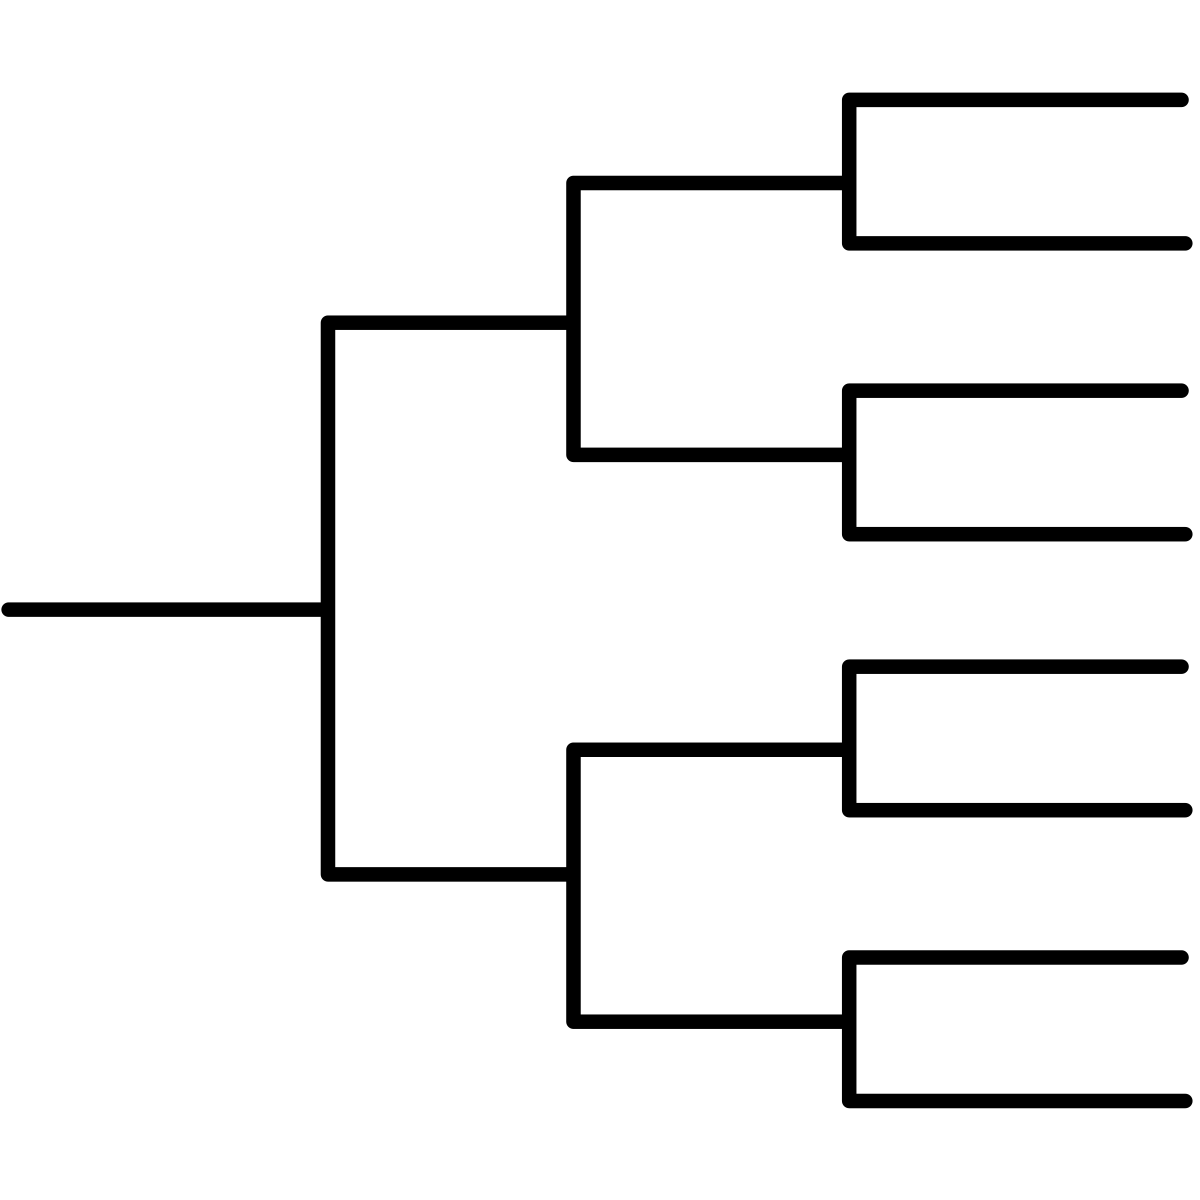
\includegraphics[width=3cm]{figures/tree.png}
      \end{figure}
  \end{columns}
\end{frame}

\begin{frame}{Ejemplo del diagrama de \'arbol}

  \begin{exampleblock}{Por ejemplo...}
    {Supongamos que vamos a comprar un helado. Entonces podemos escoger entre 3
    sabores, fresa (f), chocolate (ch) y lim\'on(l). Tambi\'en, podemos escoger entre
    cono o vaso.}
  \end{exampleblock}

\end{frame}

\begin{frame}{Ejemplo del diagrama de \'arbol}
  %%%%%%%%%%%%%%%%%%%%%%%%%%%%%%%%%%%%%%%%%%%%%%%%%%%%%%%%%%%%%
  % Se pueden poner primero los conos y despu\'es los sabores?  %
  %%%%%%%%%%%%%%%%%%%%%%%%%%%%%%%%%%%%%%%%%%%%%%%%%%%%%%%%%%%%%
  \begin{figure}[h]
    \begin{center}		
    \begin{tikzpicture}[level distance=1cm, level 1/.style={sibling distance=3cm},
      level 2/.style={sibling distance=2cm}, every node/.style={circle, draw,
      align=center} ]
          \centering
          \node[circle,draw]{}
          child{
            node{f} child{
            node{c}} child{node{v}
          } 
          }
        child{
          node{ch} child{
          node{c}} child{node{v}
          }
        }
      child{
        node{v} child{
          node{c}} child{node{v}
          }
        };
        \end{tikzpicture}
      \end{center}
      \caption{Representaci\'on en el diagrama de \'arbol}
      \label{permutaciones_tree}
  \end{figure}
\end{frame}

\begin{frame}{Permutaci\'on, variaci\'on y combinaci\'on}

  \begin{block}{Definici\'on}

    \onslide <1->Las \textbf{permutaciones y combinaciones} son maneras de representar grupos de objetos
    al seleccionarlos de un conjunto y formar subconjuntos.
    \vfill
    \onslide <2-> Las \textbf{permutaciones} se refieren a la acci\'on de ordenar u organizar los miembros de
    un conjunto en alg\'un tipo de orden o secuencia. Si un conjunto est\'a ordenado, el
    proceso de reodenar sus elementos se llama permutar.
    \vfill
    \onslide <3-> La \textbf{variaci\'on} es la disposici\'on de una parte del total de los elementos en un
    orden determinado.
    \vfill
    \onslide <4-> A diferencia de las permutaciones y variaciones, en la \textbf{combinaci\'on} no importa el orden de la
    selecci\'on de los subconjuntos.

  \end{block}

\end{frame}

\begin{frame}{Permutaci\'on, variaci\'on y combinaci\'on}

  \begin{tabular}{lcc}
    \onslide <1-> & ¿Importa el orden?  & ¿Entran todos los elementos? \\
    \hline
    \hline
    \onslide <2-> Permutaci\'on & Si                  &   Si    \\
    \onslide <3-> Variaci\'on   & Si                  &   No    \\
    \onslide <4-> Combinaci\'on & No                  &   No
  \end{tabular}

\end{frame}

\begin{frame}{Teorema de permutaciones}

  \onslide<1->
  \begin{block}{Definici\'on}
    El total de permutaciones de $n$ objetos distintos tomados de $r$ formas a la
    vez est\'a dado por:
    \begin{equation}
        P(n,r) =  \frac{n !}{(n - r)!}
    \end{equation}
  \end{block}
  \onslide<2->

  Ejemplo:
  
  \begin{figure}
    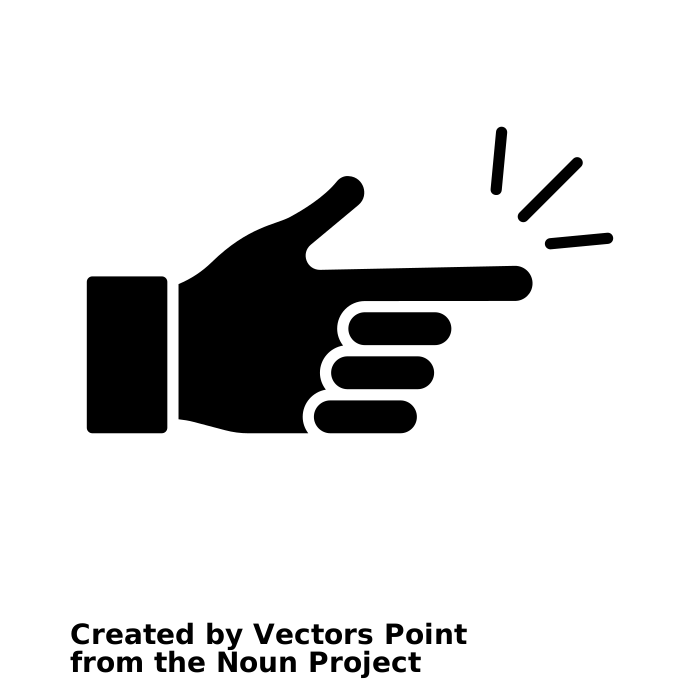
\includegraphics[width=2cm,angle=0,trim={1mm 216mm 1mm 200mm},clip]{figures/example-finger.png}
  \end{figure}

\end{frame}

\begin{frame}{Ejemplo de permutaci\'on} 

  \onslide<1->
  \begin{exampleblock}{Ejemplo}
    Encuentre el n\'umero de permutaciones del conjunto de letras $A =
    \{a,b,c,d,e,f\}$, tomando 3 al mismo tiempo. Es decir, ¿Cuantas palabras de 3
    letras podemos formar a partir de las 6 anteriores sin que se repitan?
  \end{exampleblock}
  
  \onslide<2->
  Soluci\'on:

  \begin{itemize}
    \item La primera letra podemos escogerla de 6 maneras diferentes.
    \onslide<3->\item La segunda letra podemos escogerla de 5 maneras diferentes.
    \onslide<4->\item La tercera letra podemos escogerla de 4 maneras diferentes.
  \end{itemize}
  De acuerdo a la regla de la multiplicaci\'on tenemos:
  \begin{exampleblock}{}
    \centering
    $6*5*4 = 120$
  \end{exampleblock}

\end{frame}

\begin{frame}{Ejemplo de permutaci\'on}
  Tambi\'en podemos sustituir en la f\'ormula y el resultado ser\'a el mismo:
  \begin{exampleblock}{}
    \begin{equation}
        P(n,r) =  \frac{6 !}{(6 - 3)!} = \frac{720}{6} = 120
    \end{equation}
  \end{exampleblock}
\end{frame}

\begin{frame}{Permutaci\'on con reemplazo y sin reemplazo}
  \onslide<1->
  \begin{exampleblock}{Ejemplo}
    \begin{figure}
      \raggedleft
      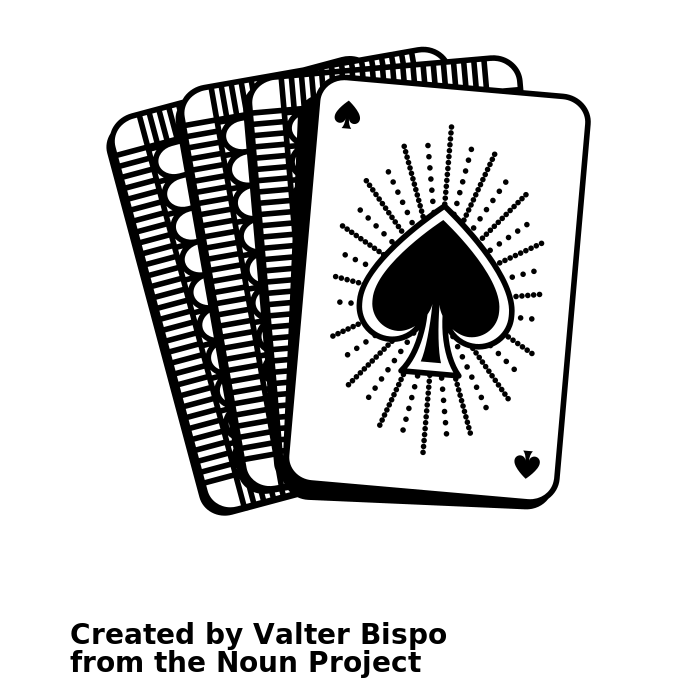
\includegraphics[width=2cm,angle=0,trim={1mm 250mm 1mm 310mm},clip]{figures/deck-of-cards.png}
    \end{figure}

    ¿De cuantas maneras posibles se pueden escoger 3 
    \\cartas de una baraja de 52
    cartas?
    \begin{itemize}
      \item Si hay reemplazo (la carta se regresa al mazo)
      \item Si no hay reemplazo (la carta no se regresa al mazo)
    \end{itemize}
  \end{exampleblock}

  \onslide<2->
  \begin{exampleblock}{Con reemplazo}
    \centering
    $52*52*52 = 52^{3} = 140 608$
  \end{exampleblock}

  \onslide<3->
  \begin{exampleblock}{Sin reemplazo}
    \centering
    $52*51*50 = 132,600$
  \end{exampleblock}

\end{frame}

\begin{frame}{Recapitulando...}
  \onslide<1->
  \begin{block}{Regla de la multiplicaci\'on}
    \begin{equation}
      n_1*n_2*n_3*...*n_k
    \end{equation}
  \end{block}

  \onslide<2->
  \begin{block}{Permutaci\'on. Muestreo con reemplazo}
    \begin{equation}
      \underbrace{n*n*n*...*n}_{r \ \text{veces}} = n^r
    \end{equation}
  \end{block}

  \onslide<3->
  \begin{block}{Permutaci\'on. Muestreo sin reemplazo.}
    \begin{equation}
      n(n-1)(n-2)...(n-r+1) = \frac {n!}{(n-r)!}
    \end{equation}
  \end{block}

\end{frame}

\begin{frame}{Permutaci\'on. Muestreo sin reemplazo.}
  
  \onslide<1->
  \begin{block}{Definici\'on}
    El total de permutaciones de $n$ objetos distintos tomados de $r$ formas a la
    vez est\'a dado por:
    \begin{equation}
        P(n,r) =  \frac{n !}{(n - r)!}
    \end{equation}
    Con el caso especial donde $n=r$, donde tenemos $n!$.
  \end{block}
  \onslide<2->
    Para deducirla a partir de la regla de la multiplicaci\'on, podemos suponer que
    $n=5$ y $r=3$, entonces observamos lo siguiente:
  
  \onslide<3->
  \begin{block}{}
    \centering
    $\overbrace{\underbrace{5*4*3}_{\text{Regla de la multiplicaci\'on}} *
    \underbrace{2*1}_{\text{lo quitamos con } (n-r)!}}^{n \ \text{factorial}}$
  \end{block}
  
\end{frame}

\begin{frame}{Permutaci\'on. Muestreo sin reemplazo.}
  
  Sustituyendo $n=5$ y $r=3$ en la f\'ormula:
  
  \begin{block}{}
    \centering
    $P(n,r) =  \frac{5 !}{(5 - 3)!} = \frac{5 !}{2!} 
            = \frac{5*4*3* \cancel{2*1}}{\cancel{2*1}} $
  \end{block}
  
\end{frame}

\begin{frame}{Permutaciones con elementos repetidos}
  \onslide<1->
  \begin{block}{Definici\'on}
    El total de permutaciones de un conjunto de $n$ objetos, de los cuales, los
    subconjuntos $n_1$, $n_2$ y $n_k$ son elementos repetidos, est\'a dado por:
  \begin{equation}
    \label{eq:permutar}
    \frac{n!}{n_{1}!*n_{2}!*...*n_{k}!}
  \end{equation}
  \end{block}

  \onslide<2->
  Ejemplo:
  \begin{figure}
    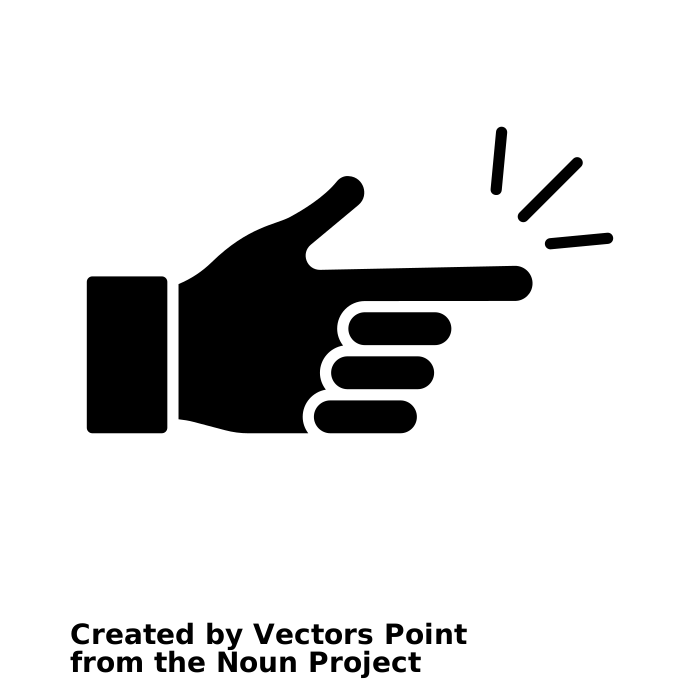
\includegraphics[width=2cm,angle=0,trim={1mm 216mm 1mm 200mm},clip]{figures/example-finger.png}
  \end{figure}
\end{frame}

\begin{frame}{Ejemplo de permutaci\'on con elementos repetidos}
  \onslide<1->
  \begin{exampleblock}{Ejemplo}
    ¿Cu\'antas palabras diferentes se pueden formar con las letras de la palabra
    \textbf{M A T E M A T I C A S}?\\
    \onslide<2->
    \textbf{Observaci\'on}:
    \begin{itemize}
      \item En total son 11 letras
      \onslide<2-> \item La letra \textbf{M} se repite 2 veces
      \onslide<3-> \item La letra \textbf{A} se repite 3 veces
      \onslide<4-> \item La letra \textbf{T} se repite 2 veces
      \onslide<5-> \item Si hacemos una permutaci\'on solo en los elementos de \textbf{M}, la palabra
      seguir\'ia siendo la misma
      \onslide<6-> \item Lo mismo con los otros elementos que se repiten
      \onslide<7-> \item Los elementos \textbf{E, I, C, S} no se repiten
    \end{itemize}
  \end{exampleblock}

\end{frame}

\begin{frame}{Soluci\'on}
  De acuerdo a la Ec. (\ref{eq:permutar}), tenemos:
  \begin{exampleblock}{}
    \centering
$\frac{11!}{\underbrace{2!}_{\textbf{M}}*\underbrace{3!}_{\textbf{A}}*\underbrace{2!}_{\textbf{T}}}
    = \frac{39916800}{2*6*2}=1663200$
  \end{exampleblock}
\end{frame}

\begin{frame}{Coeficientes binomiales}
  \onslide<1->
  \begin{block}{Definici\'on}
    Para cualquier entero positivo $k$ y $n$, el coeficiente binomial
    $\binom{n}{k}$, que se lee \textit{n combinaci\'on k}, es el n\'umero de
    subconjuntos de tamaño $k$ de un conjunto de tamaño $n$. Se puede calcular de la
    siguiente manera:
    \onslide<2->
  \begin{equation}
    \binom{n}{k} = \frac{n(n-1)...(n-k+1)}{k!} = \frac{n!}{(n-k)!k!}
    \label{eq:binomial}
  \end{equation}
  \onslide<3->
  Para $k>n$, $\binom{n}{k}=0$ \\
  \onslide<4->
  \textbf{Observaci\'on}\\
  \begin{itemize}
    \item $\frac{n!}{(n-k)}$ es la permutaci\'on sin reemplazo.
    \onslide<5-> \item Ya que no nos importa que los elementos est\'en ordenados,
    podemos quitar aquellos subconjuntos cuyos elementos se repitan. Esto lo hacemos
    dividiendo entre $k!$.
  \end{itemize}
\end{block}
\end{frame}

\begin{frame}{Ejemplo de uso del coeficiente binomial}
  \onslide<1->
  \begin{exampleblock}{Conjunto potencia}
Dado el conjunto $A =\{a,b,c,d\}$, ¿Cu\'antos subconjuntos podemos formar con
0, 1, 2, 3, y 4 elementos?
  \end{exampleblock}
  \onslide<2->
  \begin{exampleblock}{}
    \centering
    $ P(A) = \binom{4}{0} + \binom{4}{1} + \binom{4}{2} + \binom{4}{3} + \binom{4}{4} $
  \end{exampleblock}
  \onslide<3->
  Que de acuerdo con la Ec. (\ref{eq:binomial}):

  \begin{exampleblock}{}
    \centering
  $ P(A) = \frac{4!}{(4-0)!0!} + \frac{4!}{(4-1)!1!} + \frac{4!}{(4-2)!2!} + \frac{4!}{(4-3)!3!} + \frac{4!}{(4-4)!4!} $
  \end{exampleblock}
  \onslide<5->
  \begin{exampleblock}{}
    \centering
  $ P(A) = \frac{4!}{(4)!0!} + \frac{4!}{(3)!1!} + \frac{4!}{(2)!2!} + \frac{4!}{(1)!3!} + \frac{4!}{(0)!4!} $
  \end{exampleblock}

\end{frame}

\begin{frame}{Ejemplo de uso del coeficiente binomial}

  \begin{exampleblock}{Conjunto potencia}
    Dado el conjunto $A =\{a,b,c,d\}$, ¿Cu\'antos subconjuntos podemos formar con 0,
    1, 2, 3, y 4 elementos?
  \end{exampleblock}
  
  Podemos calcular los subconjuntos de 0, 1, 2, 3 y 4 elementos de la siguiente
  forma:

  \begin{exampleblock}{}
    \centering
    $ P(A) = \binom{4}{0} + \binom{4}{1} + \binom{4}{2} + \binom{4}{3} + \binom{4}{4} $
  \end{exampleblock}
  \onslide<1->
  \begin{exampleblock}{}
    \centering
    $ P(A) = 1 + 4 + 6 + 4 + 1 $
  \end{exampleblock}
  \onslide<2->
  Por lo que tenemos un total de:
  \begin{exampleblock}{}
    \centering
    $ P(A) = 16 \text{ subconjuntos de } A$
  \end{exampleblock}

\end{frame}

\begin{frame}
  \onslide<1->
  \begin{exampleblock}{Observaci\'on}
    De acuerdo a: 
    \centering
    $ P(A) = \binom{4}{0} + \binom{4}{1} + \binom{4}{2} + \binom{4}{3} +
    \binom{4}{4} $ \\
    \ \\
    De donde obtenemos:
    $ P(A) = 1 + 4 + 6 + 4 + 1 $
  \end{exampleblock}
  \onslide<2->
  Observamos que:
  
  \begin{exampleblock}{}
    \centering
    $\binom{4}{1} = \binom{4}{3}$
  \end{exampleblock}
  
  \onslide<3->
  Sin embargo, computacionalmente:

  \begin{exampleblock}{}
    \centering

    $\binom{4}{1} = \frac{4}{1}$\\
    \ \\

    $\binom{4}{3} = \frac{4*3*2}{3*2*1}$
  \end{exampleblock}
  \onslide<4->
  Por lo que:
  \begin{exampleblock}{}
    \centering
    $\binom{4}{1}$ ahorra tiempo y espacio.
  \end{exampleblock}
\end{frame}

\begin{frame}
  \begin{block}{De lo anterior, podemos concluir que:}
    \begin{equation}
      \binom{n}{n-r} = \binom{n}{r}
    \end{equation}
  \end{block}
  En otras palabras:
  \begin{block}{}
    Si $a+b=n$, entonces $\binom{n}{a} = \binom{n}{b}$
  \end{block}
\end{frame}

\begin{frame}
  \onslide<1->
    Retomemos $\binom{4}{3}$ del conjunto $A=\{a,b,c,d\}$, tendremos las
    siguientes permutaciones y combinaciones: \\
\ \\

\begin{center}
\begin{tabular}{cc}
  \onslide<2-> \textbf{Combinaciones } & \textbf{Permutaciones }\\
  \hline
  \onslide<3-> abc & abc,acb,bac,bca,cab,cba \\
  \hline
  \onslide<4-> abd & abd,adb,bad,bda,dab,dba \\
  \hline
  \onslide<5-> acd & acd,adc,cad,cda,dac,dca \\
  \hline
  \onslide<6-> bcd & bcd,bdc,cbd,cdb,dbc,dcb

\end{tabular}
\end{center}

\end{frame}

\end{document}


